\documentclass{article}
\usepackage{graphicx}
\usepackage{float}
\usepackage{amsmath}
\usepackage{lastpage}
\usepackage[margin=0.85in]{geometry}
\usepackage{fancyhdr}
\pagestyle{fancy}
\lhead{CSC373 Summer 2015}
\chead{Tutorial 5}
\rhead{TA: Eric Zhu}
\cfoot{Page \thepage~of~\pageref{LastPage}}
%\setlength{\parindent}{0pt}
\begin{document}

\section{Ford-Fulkerson}
Consider the following flow network $G$.
Compute a maximum flow in this network, using the Ford-Fulkerson
algorithm.

\begin{figure}[H]
\centering
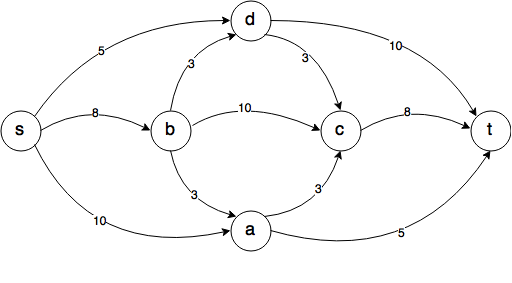
\includegraphics[width=0.8\textwidth]{g_0.png}
\caption{A flow network $G$}
\end{figure}

Let's start with constructing the residual flow network $G_f$.
The initial residual flow network looks just the same as the graph diagram
above. However, the number on each edge now represents the {\it unused
capacity} - the maximum amount of flow that can be pushed through the edge.
It is important to note that the flows in the residual network $G_f$ are not
real flows - not in the same sense as the actual flows in $G$.
You can think of $G_f$ as a data storage for storing the intermediate steps.

We look for an $s \rightarrow t$ path in this network, and
we find the path $s \rightarrow b \rightarrow c \rightarrow t$.

\begin{figure}[H]
\centering
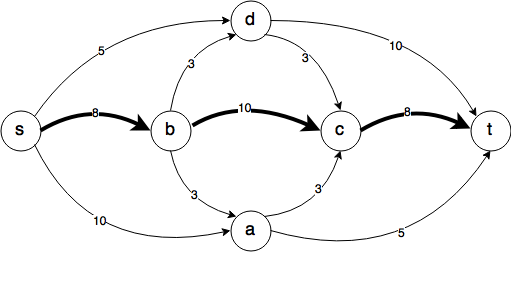
\includegraphics[width=0.8\textwidth]{gf_0.png}
\caption{Picking an $s \rightarrow t$ path on the residual network $G_f$}
\end{figure}

The edges with minimum unused capacity on this path are $s \rightarrow b$
and $c \rightarrow t$, both have unused capacity 8. So we push amount of
flow 8 through this path.
Now we update the residual network $G_f$:
\begin{itemize}
\item Update forward edges on this path with the new unused capacities
- substracting each original unused capacity with the amount of flow 
pushed through this path. If the unused capacity was reduced to 0 for an edge,
we simply remove the edge from the network. 
\item Add a backward edge for every forward edge on this path.
Each new backward edge will have unused capacity equals to the amount of
flow pushed through this path. If a backward edge already exists for a
forward edge, add the amount of flow pushed to the unused capacity of the
backward edge.
\end{itemize} 
Basically, we use forward edge to store the ``left-over'' capacity,
and backward edge to store the ``surplus'' capacity that can be
reversed in the future when the backward edge becomes an forward edge in
a new $s \rightarrow t$ path.

\begin{figure}[H]
\centering
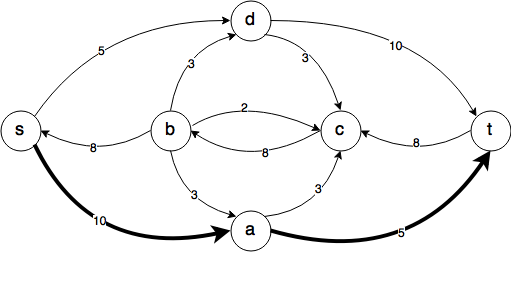
\includegraphics[width=0.8\textwidth]{gf_1.png}
\caption{On $G_f$, update path $s \rightarrow b \rightarrow c \rightarrow t$, then pick a new $s \rightarrow t$ path
$s \rightarrow a \rightarrow t$}
\end{figure}

After updating $G_f$, we look for a new $s \rightarrow t$ path in this 
network. We use the path $s \rightarrow a \rightarrow t$.
We can push amount of flow 5 through this path.
Update the forward edges on this path and add backward edges with
new unused capacities.

\begin{figure}[H]
\centering
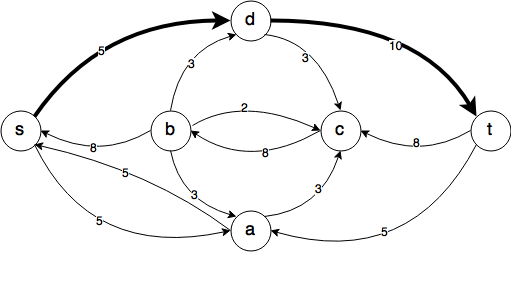
\includegraphics[width=0.8\textwidth]{gf_2.png}
\caption{On $G_f$, update path $s \rightarrow a \rightarrow t$, then pick a new path
$s \rightarrow d \rightarrow t$}
\end{figure}

We find another $s \rightarrow t$ path: $s \rightarrow d \rightarrow t$
to push amount of flow 5.
Update the forward edges on this path and add backward edges with new
unused capacities.

\begin{figure}[H]
\centering
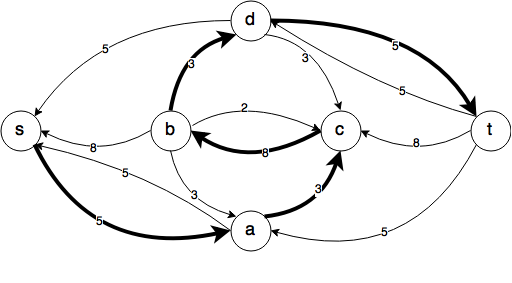
\includegraphics[width=0.8\textwidth]{gf_3.png}
\caption{On $G_f$, update path $s \rightarrow d \rightarrow t$, 
then pick a new path $s \rightarrow a \rightarrow c \rightarrow b
\rightarrow d \rightarrow t$}
\end{figure}

We find yet another path: $s \rightarrow a \rightarrow c \rightarrow b
\rightarrow d \rightarrow t$. The maximum amount of flow we can push
through this path is 3, because the minimum unused edge capacity in this 
path is 3 (edges $a \rightarrow c$ and $b \rightarrow d$).
Note the edge $b \rightarrow c$, it was a backward edge in the path
$s \rightarrow b \rightarrow c \rightarrow t$ which we picked in the first
step, and now it becomes a forward edge in the current path.
So by pushing flow through the current path, we are reversing the 
``surplus'' flow in the original edge $b \rightarrow c$.

\begin{figure}[H]
\centering
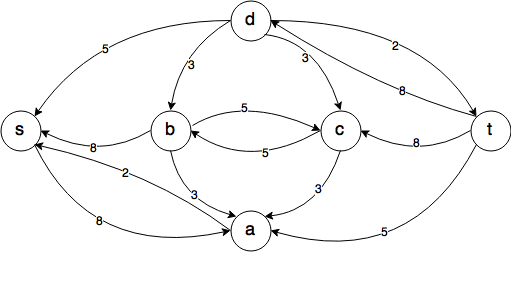
\includegraphics[width=0.8\textwidth]{gf_4.png}
\caption{On $G_f$, update path $s \rightarrow a \rightarrow c \rightarrow b
\rightarrow d \rightarrow t$, no more $s \rightarrow t$ path}
\end{figure}

After updating the last path, we cannot find any more $s \rightarrow t$
path in the residual network $G_f$. The total amount of flow we have pushed
is $8 + 5 + 5 + 3 = 21$. According to the Ford-Fulkerson algorithm, this
is the maximum flow in this network.

\section{Cut Capacity and Flow}
Consider the cut $X_0 = (\{s,b,c,d\}, \{a,t\})$. Identify all forward and
all backward edges across $X_0$, then compute the capacity and the flow
across $X_0$.

Let's first label the original network $G$ with the result we obtained from
the final residual network $G_f$. 
On $G_f$, each reverse edge (reverse w.r.t. $G$) 
stores the flow through the corresponding original edge on $G$.
We label each edge on $G$ with the amount of flow and capacity.

\begin{figure}[H]
\centering
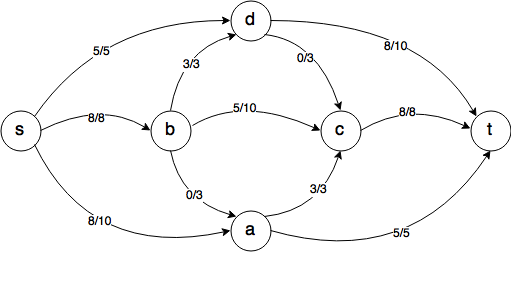
\includegraphics[width=0.8\textwidth]{g_1.png}
\caption{Label edges in $G$ with [flow]/[capacity]}
\end{figure}

Now let's find the cut $X_0 = (\{s,b,c,d\}, \{a,t\})$.

\begin{figure}[H]
\centering
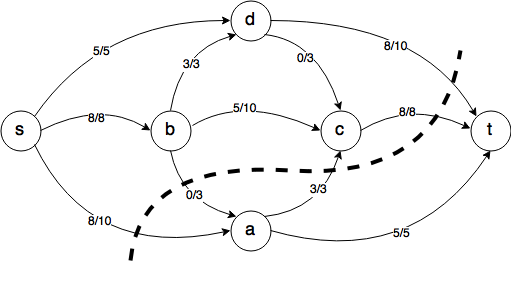
\includegraphics[width=0.8\textwidth]{g_2.png}
\caption{The cut $X_0 = (\{s,b,c,d\}, \{a,t\})$}
\end{figure}

The cut separate nodes in the network into two groups:
$V_s = \{s, b, c, d\}$ and $V_t = \{a, t\}$. The forward edges are defined
as the edges going from $V_s$ to $V_t$, and the backward edges are defined
as the edges going from $V_t$ to $V_s$. 
Note the terms ``forward edges''
and ``backward edges'' are different from the ones we used in the last section.
Here they refer to edges on the original network $G$.
\begin{itemize}
\item Forward edges: $\{s \rightarrow a,~ b \rightarrow a,~ c \rightarrow t,~
d\rightarrow t\}$
\item Backward edges: $\{a \rightarrow c\}$
\end{itemize}

The capacity of the cut $X_0$ is:
\begin{equation}
	\begin{split}
		c(X_0) &= \sum_{e_i \in forward~edges} c(e_i)\\
		&=c(s \rightarrow a) + c(b \rightarrow a) + 
		c(c \rightarrow t) + c(d\rightarrow t)\\
		&= 10 + 3 + 8 + 10 \\
		&= 31
	\end{split}
\end{equation}

The flow across the cut $X_0$ is:
\begin{equation}
	\begin{split}
		f(X_0) &= \sum_{e_i \in forward~edges} f(e_i)
		- \sum_{e_i \in backward~edges} f(e_i)\\
		&= f(s \rightarrow a) + f(b \rightarrow a) + 
		f(c \rightarrow t) + f(d\rightarrow t) - f(a \rightarrow c)\\
		&= 8+0+8+8-3\\
		&= 21
	\end{split}
\end{equation}

{\bf Remember}, 
when looking for the forward and backward edges of a cut, always work on the
original network $G$. 
The edges and labels on the residual network $G_f$ 
are not real edges and not real flows.

\section{Minimum Cut}
Find a cut in the network above whose capacity is equal to the value
of your maximum flow (this provides a guarantee that your flow really
is maximum). Use the algorithm outlined in the proof of the
Ford-Fulkerson theorem.

Start with $X_1 = (\{s\}, \{a,b,c,d,t\})$ and flow from before.
Edge $s \rightarrow a$ crosses cut forward with residual capacity 2, so set
$X_1 = (\{s,a\}, \{b,c,d,t\})$. Now no more forward edge acrosses the cut 
with residual capacity - all the forward edges across the cut are used at
their full capacities.

As before, the capacity of the cut $X_1$ is:
\begin{equation}
	\begin{split}
		c(X_1) &= \sum_{e_i \in forward~edges} c(e_i)\\
		&=c(s \rightarrow b) + c(s \rightarrow d) + 
		c(a\rightarrow c) + c(a \rightarrow t)\\
		&= 8 + 5 + 3 + 5 \\
		&= 21
	\end{split}
\end{equation}

The flow across the cut $X_1$ is:
\begin{equation}
	\begin{split}
		f(X_1) &= \sum_{e_i \in forward~edges} f(e_i)
		- \sum_{e_i \in backward~edges} f(e_i)\\
		&= f(s \rightarrow b) + f(s \rightarrow d) + 
		f(a \rightarrow c) + f(a\rightarrow t) - f(b \rightarrow a)\\
		&=8 + 5 + 3 + 5 -0\\
		&= 21
	\end{split}
\end{equation}

Since $f(X_1) = c(X_1)$, $X_1$ is a minimum cut of $G$.

An alternative way to find the minimum cut in $G$ is to look for ``blocking edges'' in
the residual network $G_f$: starting with 
$V_s = \{s\}$ and $V_t = \{a, b, c, d, t\}$,
do Depth-First Search starting from $s$ and keep track of visited nodes: 
whenever a node $n$ (other than $s$) is reached, $V_s = V_S \cup \{n\}$,
and stops when no more out-going path that leads to un-visited node 
can be find for the current node -- ``blocked'' by the in-coming edges.
The resulting $V_s$ and $V_t$ form a minimum cut.

\section{Multi-source and Multi-sink Network}
Explain carefully how to solve the maximum flow problem in a
multi-source, multi-sink network -- one where there can be more than one
source $s_1,~...,~s_k$ and more than one sink $t_1,~...,~t_l$. Justify that your
solution is correct.

{\bf Solution} 
Add ``super-source'' $s$ with edges $s \rightarrow s_1,~...,~s\rightarrow s_k$
each of capacity $\inf$; add ``super-sink'' $t$ with edges 
$t_1 \rightarrow t,~...,~ t_l \rightarrow t$ each of capacity $\infty$. 
(Instead of using $\infty$, can set capacity to sum of outgoing/incoming
capacities).

Max flow in resulting network $=$ max flow in original network because:
\begin{itemize}
\item Any flow in original network can be extended to a flow in resulting
network (for new edges from super-source to source, set flow equal to
total flow out of source; for new edges from sink to super-sink, set
flow equal to total flow into sink) -- hence, max flow in new network
$\ge$ max flow in original network;
\item Any flow in resulting network induces flow in original network (flow
out of every source and into every sink limited only by edges in
original network because of "infinite" capacities on new edges) -- 
hence, max flow in original network $\ge$ max flow in new network.
\end{itemize}

\end{document}
